\documentclass[12pt,b5paper]{report}
\usepackage[margin=1in]{geometry}
\usepackage{graphicx} % embed images
\graphicspath{ {images/} }
\usepackage{url} %for proper url entries

\usepackage{tikz}
\usetikzlibrary{calc}
\newcommand\HRule{\rule{\textwidth}{1pt}}

\usepackage{fancyhdr}
\usepackage{fancyvrb}
\usepackage{color}
\usepackage[utf8]{inputenc}
\usepackage{float}
\usepackage{minted}
\usepackage{listings}
\lstset{
         basicstyle=\footnotesize\ttfamily, 
         numberstyle=\tiny,          
         numbersep=5pt,             
         tabsize=2,                
         extendedchars=true,      
         breaklines=true,        
         showspaces=false,      
         showtabs=false,       
         xleftmargin=17pt,
         framexleftmargin=17pt,
         framexrightmargin=5pt,
         framexbottommargin=4pt,
         showstringspaces=false 
 }
 \lstloadlanguages{
         python,
         javascript
 }

\begin{document}

\renewcommand\bibname{References} %Renames "Bibliography" to "References" on ref page
\pagenumbering{gobble}

\topskip0pt
\vspace*{\fill}

\begin{center}

\fontsize{14pt}{12pt}\selectfont
Project Report

\hspace{0.7em}

on

\hspace{0.7em}
\vspace{0.3in}

\fontsize{20pt}{12pt}\selectfont{\bfseries{Image Super Resolution\\ using Deep Neural Networks}}

\hspace{1em}
\vspace{0.3in}

submitted by

\hspace{1em}
\vspace{0.3in}

\fontsize{14pt}{12pt}\selectfont
Aayisha A A ( 12150076 )\\
Abhai Kollara ( 12150002 )\\
Abin Simon ( 12150005 )\\
Mohammed Fayis P T ( 12150043 )

\hspace{1em}
\vspace{0.5in}

\normalsize
In partial fulfillment of the requirements for the award of degree of Bachelor of Technology in Computer Science and Engineering.

\hspace{1em}
\vspace{0.5in}

\fontsize{15pt}{12pt}\selectfont
DIVISION OF COMPUTER ENGINEERING\\
SCHOOL OF ENGINEERING\\
COCHIN UNIVERSITY OF SCIENCE AND TECHNOLOGY

\hspace{1em}

\normalsize
NOVEMBER 2017
\end{center}

\vspace*{\fill}
\newpage
\centerline{\large{\bfseries{ACKNOWLEDGEMENT}}}

\hspace{1in}

\normalsize

We take this opportunity to express our profound gratitude and deep regards to our guide \textbf{Mrs Deepa Paul}
,for providing us with the right guidance and advice at the crucial junctures and for her constant encouragement throughout the course of this project's design. We are highly indebted to \textbf{Associate Prof. Pramod Pavithran}
 , Division of Computer Science our batch coordinator for his constant supervision and support for completing the project. We extend our sincere thanks to our respected Head of the department, \textbf{Associate Prof. Damodaran.V}
 ,Head of Division,Division of Computer Science and all other faculty members of for sharing their valuable time and knowledge with us. We thank God, the almighty for blessing us with his grace and taking our endeavour to a successful culmination. Lastly we would like to thank my friends and family for their constant encouragement without which this project would not have been possible.

\newpage
\centerline{\large{\bfseries{DECLARATION}}}

\hspace{1in}

\normalsize

We, Miss Aayisha A A, Mr. Abhai Kollara, Ms. Abin Simon & Ms.Mohammed Fayis P T  hereby declare that this project is the record of authentic work carried out by us during the academic year 2017 - 2018 and has not been submitted to any other University or Institute towards the award of any degree.

\begin{flushright} Abin Simon\\
Aayisha A A\\
Abhai Kollara\\
Mohammed Fayis P T
\end{flushright}

\newpage
\centerline{\large{\bfseries{ABSTRACT}}}

\hspace{1in}

\normalsize

In most digital imaging applications, high resolution images or videos are usually desired for later image processing and analysis. The desire for high image resolution stems from two principal application areas: improvement of pictorial information for human interpretation; and helping representation for automatic machine perception. Image resolution describes the details contained in an image, the higher the resolution, the more image details.
Super-resolution (SR) are techniques that construct high-resolution (HR) images from several observed low-resolution (LR) images, thereby increasing the high frequency components and removing the degradation caused by the imaging process of the low resolution camera. The basic idea behind SR is to combine the non-redundant information contained in multiple low- resolution frames to generate a high-resolution image. A closely related technique with SR is the single image interpolation approach, which can be also used to increase the image size. However, since there is no additional information provided, the quality of the single image interpolation is very much limited due to the ill-posed nature of the problem, and the lost frequency components cannot be recovered. In the SR setting, however, multiple low-resolution observations
are available for reconstruction, making the problem better constrained. The non-redundant information contained in the these LR images is typically introduced by subpixel shifts between them. These subpixel shifts may occur due to uncontrolled motions between the imaging system and scene, e.g., movements of objects, or due to controlled motions, e.g., the satellite imaging system orbits the earth with predefined speed and path.
In our project we attempt to use deep convolutional neural nets to train a model to output enlarged images given a picture. We also attempt to exploit generative-adverserial nets in favour of this project.

\pagenumbering{roman} %numbering before main content starts
\tableofcontents
\listoffigures

\pagestyle{fancy}
\fancyhf{}
\rhead{Image Super-resolution}
\lhead{}
\rfoot{Page \thepage}
\lfoot{Department of Computer Science and Engineering}

\newpage
\pagenumbering{arabic} %reset numbering to normal for the main content

\chapter{Introduction}

We in the current days, with the ever increasing number of phones which have cameras take a lot more photos than we used to take in the past. But the main issue with the photos is that a lot of them that we take using our phones are of very low resolution since phone cameras even though has evolved a lot still has a lot of way to go when it comes to high resolution images as the camera technology is not that advanced just yet and also due to the fact that we have to shrink the cameras into a small form factor so as to make it fit into a small device like a phone. 

Our project proposes a way in which we can improve the image clarity with the use of neural networks so that it allows us to have sharper images with more detail. We use neural networks to learn a feature representation of the image and try to reconstruct an enhanced image from the condensed representation.

It also is highly useful when we have images from the past which could not have been taken using better cameras as they didn't even exist back then.

\chapter{Literature Survey}

\section{Paper Analysis}
For our platform to form we had to take assistance from already explored thesis and paper.They provided us with basic understanding and different aspects of interpretation of modern traffic problem.The guides we used to expand our platform includes.

\begin{figure}[htb]
    \centering
    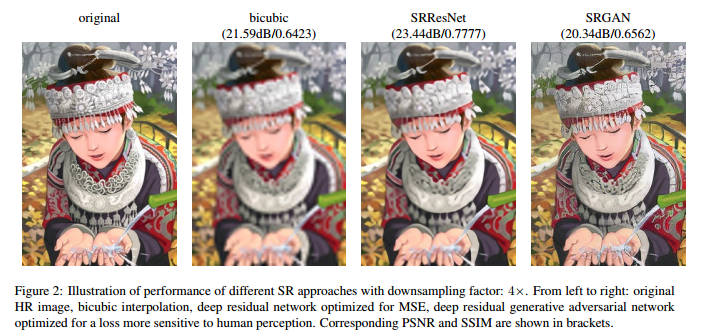
\includegraphics[width=\linewidth]{srdiff.jpg}
    \caption{Better edge correction}
    \label{fig:srdiff} % insert suitable label, this is used to refer to a fig from within the text
\end{figure}

Deep Learning-based methods are currently active and showing significant performances on SISR tasks. Super-Resolution Convolutional Neural Network (SRCNN) is the method proposed at this very early stage. C. Dong et al.use 2 to 4 CNN layers to prove that the learned CNN layers model performs well on SISR tasks. The authors concluded that using a larger CNN filter size is better than using deeper CNN layers. SRCNN is followed by Deeply-Recursive Convolutional Network for Image Super-Resolution (DRCN). DRCN uses deep (a total of 20) CNN layers, which means the model has huge parameters. However, they share each CNN’s weight to reduce the number of parameters to train, meaning they succeed in training the deep CNN network and achieving significant performances. The other Deep Learning based method VDSR is proposed by the same authors of DRCN. VDSR uses Deep Residual Learning, which was developed by researchers from Microsoft Research and is famous for receiving first place in ILSVRC 2015 (a large image classification competition). By using residual-learning and gradient clipping, VDSR proposed away of significantly speeding up the training step. Very deep Residual Encoder-Decoder Networks(RED) are also based on residual-learning. RED contains symmetric convolutional(encoder) and deconvolutional(de-coder)layers. It also has skip connections and connects instead to every two or three layers. Using this symmetric structure, they can train very deep (30 of) layers and achieve state-of-the-art performance. These studies therefore reflect the trendof “the Deeper the Better”. Onthe other hand, Yaniv Romano et al. proposed Rapid and Accurate Image Super Resolution (RAISR) , which is a shallow and faster learning-based method. It classifies input image patches according to the patch’s angle, strength and coherence and then learn maps from LR image to HR image among the clustered patches. C. Dong et al. also proposed FSRCNN as a faster version of their SRCNN .FSRCNN uses transposed CNN to process the input image directly. RAISR and FRSCNN’s processing speeds are 10 to 100 times faster than other state-of-the-art Deep Learning-based methods. However, their performance is not as high as other deeply convolutional methods,like DRCN, VDSR orRED.

\subsection{Fast and Accurate Image Super Resolution by Deep CNN with Skip Connection and Network in Network}
In this paper the authors propose a highly efficient and faster Single Image Super Resolution (SISR) model with Deep Convolutional neural networks (Deep CNN) . Deep CNN have recently shown that they have a significant reconstruction performance on single image super resolution. The current trend is using deeper CNN layers to improve performance . However , deep models demand larger computation resources and are not suitable for network edge devices like mobile, tablet and IoT devices . Our model achieves state of the art reconstruction performance with at least 10 times lower calculation cost by Deep CNN with Residual Net, Skip Connection and Network in Network (DCSCN) . A combination of Deep CNNs and Skip connection layers are used as a feature extractor for image features on both local and global areas . Parallelized 1x1 CNN s, like the one called Network in Network , are also used for image reconstruction . That structure reduces the dimensions of the previous layer ’s output for faster computation with less information loss , and make it possible to process original images directly . Also w e optimize the number of layers and filters of each CNN to significantly reduce the calculation cost . Thus, the proposed algorithm not only achieves state of the art performance but also achieve s faster and more efficient computation .

\begin{figure}[htb]
    \centering
    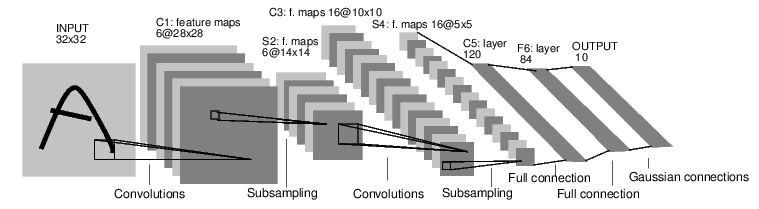
\includegraphics[width=\linewidth]{fe.png}
    \caption{Feature Extraction}
    \label{fig:fe} % insert suitable label, this is used to refer to a fig from within the text
\end{figure}

\subsection{Photo-Realistic Single Image Super-Resolution Using a Generative Adversarial Network}
Despite the breakthroughs in accuracy and speed of single image super-resolution using faster and deeper con- volutional neural networks, one central problem remains largely unsolved: how do we recover the finer texture details when we super-resolve at large upscaling factors? The behavior of optimization-based super-resolution methods is principally driven by the choice of the objective function. Recent work has largely focused on minimizing the mean squared reconstruction error. The resulting estimates have high peak signal-to-noise ratios, but they are often lacking high-frequency details and are perceptually unsatisfying in the sense that they fail to match the fidelity expected at the higher resolution. In this paper, the authors introduce SRGAN, a generative adversarial network (GAN) for image super- resolution (SR). To our knowledge, it is the first framework capable of inferring photo-realistic natural images for 4 × upscaling factors. To achieve this, we propose a perceptual loss function which consists of an adversarial loss and a content loss. The adversarial loss pushes our solution to the natural image manifold using a discriminator network that is trained to differentiate between the super-resolved images and original photo-realistic images. In addition, they use a content loss motivated by perceptual similarity instead of similarity in pixel space. The deep residual network is able to recover photo-realistic textures from heavily downsampled images on public benchmarks. An extensive mean-opinion-score (MOS) test shows hugely significant gains in perceptual quality using SRGAN. The MOS scores obtained with SRGAN are closer to those of the original high-resolution images than to those obtained with any state-of-the-art method.

\subsection{Image Super-Resolution Using Deep Convolutional Networks}
They propose a deep learning method for single image super-resolution (SR). Their method directly learns an end-to-end mapping between the low/high-resolution images. The mapping is represented as a deep convolutional neural network (CNN) that takes the low-resolution image as the input and outputs the high-resolution one. They further show that traditional sparse-coding-based SR methods can also be viewed as a deep convolutional network. But unlike traditional methods that handle each component separately, our method jointly optimizes all layers. Their deep CNN has a lightweight structure, yet demonstrates state-of-the-art restoration quality, and achieves fast speed for practical on-line usage. They explore different network structures and parameter settings to achieve trade-offs between performance and speed. Moreover, they extend our network to cope with three color channels simultaneously, and show
better overall reconstruction quality.

% \chapter{Feasibility study}

The design of the module for image super resolution is quite challenging, considering that various kinds of technical aspects involved in this project. The project has a multitude of problems that it will have to deal with. The main challenge is the issue that the system has to have a generic system that will be able to deal with the inputs that the system gets.

Having a good sample training set is really vital for such kind of an approach so as to obtain the maximum accuracy in the output. Since this is not so much of an issue as we can easily create large amount of data set from a lot of good quality images. The main issue with the dataset is having to deal with the diversity of the images as we need to have a wide range of data point to make it working as a general system.

In this Project, we demonstrate how image processing, and machine learning can be used to enhance the clarity of an image. To that end, we propose two segments: one is an image processing part, and the other is a neural network modal that will work on that image and fix image issues.

The proposed system will follow the below given processing model to enhance image.

\begin{itemize}
    \item The image will can be uploaded from the device, both computer or a mobile
    \item The obtained image is then sent to a sever
    \item A small amount of preprocessing is done on the image
    \item The images if processed using the image super resolution model
    \item Result is sent back to the device
    \item The image that has been enhanced in the server is made available to the user via the UI
\end{itemize}

\chapter{Problem statement}


The goal of super resolution (SR) is to produce a high resolution image from a low resolution input. Rather than simply interpolating the unknown pixel values we wish to infer their true value based on the information in the input. To do this we introduce the super resolution equation.

\begin{figure}[htb]
    \centering
    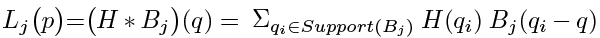
\includegraphics[width=\linewidth]{eq1.png}
    \caption{Super resolution}
    \label{fig:eq1} % insert suitable label, this is used to refer to a fig from within the text
\end{figure}


Where $Lj(p)$ denotes the value of the pixel at location p in the low resolution image. Similarly $H(q)$ denotes the value at pixel location q in the latent high resolution image. $B(.)$ is the blur kernel, or point spread function (PSF). The subscript j denotes a particular low-res image and blur kernel, which will be described later. Equation states that the low resolution image is assumed to be the result of a convolution between the high resolution image and a PSF and then down-sampled.

\begin{figure}[htb]
    \centering
    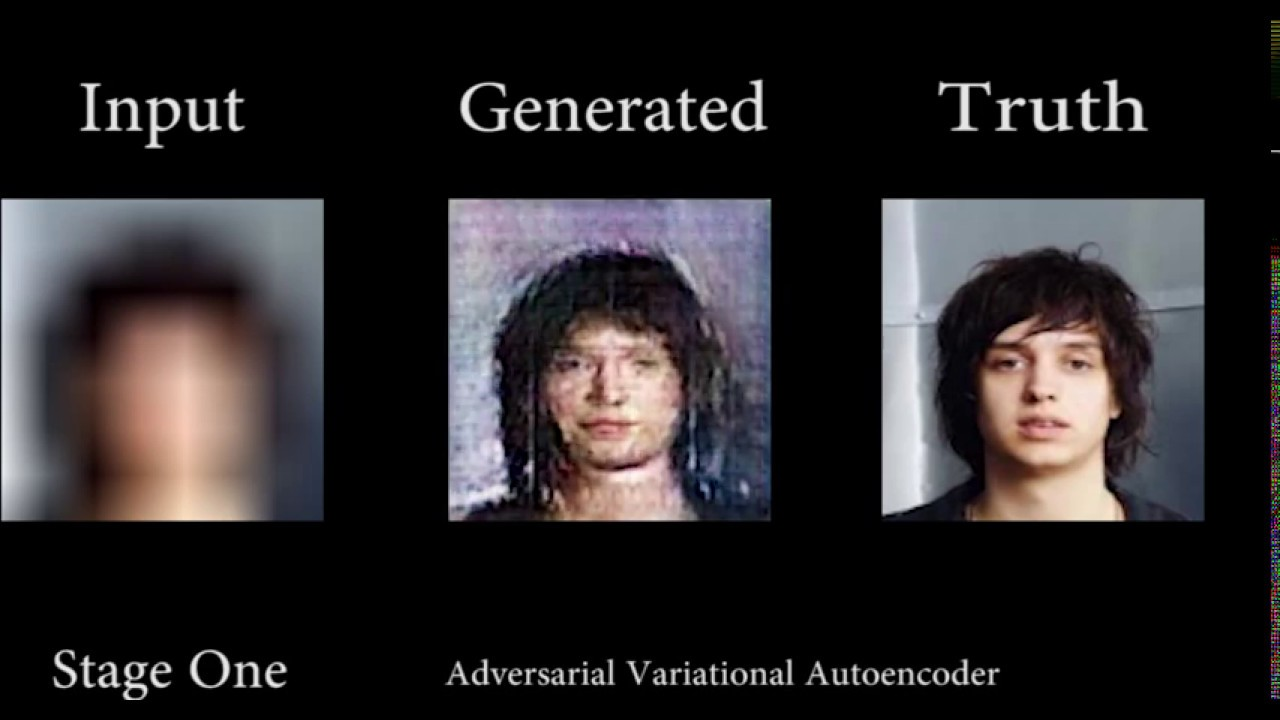
\includegraphics[width=\linewidth]{sr4.jpg}
    \caption{Better edge correction}
    \label{fig:sr4} % insert suitable label, this is used to refer to a fig from within the text
\end{figure}

Because convolution is a linear operation the above equation induces a set of linear constraints on the latent high resolution image H. Given only a single low resolution image, though, the equation is underconstrained.

Using the concept of patch redundancy it is possible to at least approximate a solution to the equation using only a single image. In D. Glasner, S. Bagon, M. Irani the authors present an algorithm for performing super resolution from a single image. This project implements the specified algorithm and presents results on a set of images.


\chapter{System study}

\section{Current System}
Most of the current systems make use of techniques like interpolation to achieve super resolution. The surge of recent neural networks has produced several research papers making use of neural networks to achieve image superresolution. Almost all of them use convolutional neural networks to extract features hierarchically. Transposed convolutions can be used to recreate the enhanced image from the extracted features.

\begin{figure}[htb]
    \centering
    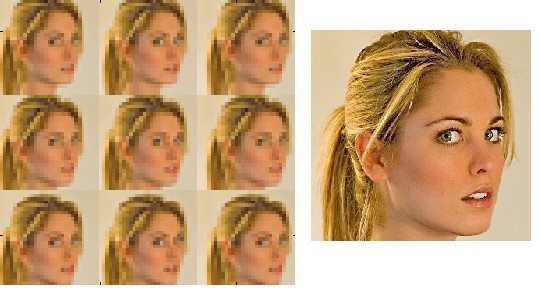
\includegraphics[width=\linewidth]{multi_sample.jpg}
    \caption{Multiple sample based approch}
    \label{fig:ms} % insert suitable label, this is used to refer to a fig from within the text
\end{figure}

\subsection{Interpolation based approach}
Interpolation-based SR algorithms construct a HR image by projecting all the acquired LR images to a reference image. All the information available from each image is then fused together, due to the fact that each LR image provides an amount of additional information about the scene, and finally a deblurring process is applied to the obtained image. 

\subsection{Frequency-domain-based approach}
A major class of multi-frames SR methods utilizes a frequency domain formulation of the SR problem. The main principle is that clues ab out high frequencies are spread across the multiple LR images in form of aliased spectral frequencies. The first frequency-domain SR method can b e credited to Tsai and Huang [8], who considered SR reconstruction from noise-free LR images. They proposed of first transform the LR image data into the Discrete Fourier Transform (DFT) domain, and then combine them according to the relationship between the aliased DFT coeffcients of the observed LR images. The approach is based on the following principles:

1. The shifting prop erty of the Fourier transform
2. The aliasing relationship b etween the continuous Fourier transform (CFT) and the DFT of observed LR images
3. The assumption that an original HR image is band-limited.

\section{Proposed System}

\begin{figure}[htb]
    \centering
    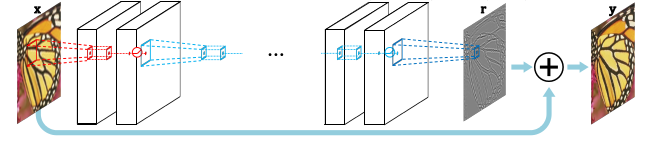
\includegraphics[width=\linewidth]{acc.png}
    \caption{Accurate Image Super Resolution}
    \label{fig:acc} % insert suitable label, this is used to refer to a fig from within the text
\end{figure}

We propose a novel super resolution method using neural networks to learn feature representations of images and then recreate enhanced versions of the image using these representations. While there are several neural networks based approaches already in place we attempt to use capsule networks to learn feature representations instead of convolutional neural networks. Capsule networks have been shown to produce slightly better results than the current goto choice of convolutional neural networks.

\begin{figure}[htb]
    \centering
    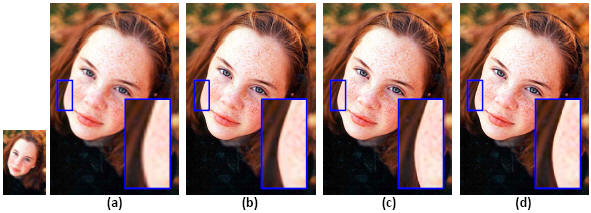
\includegraphics[width=\linewidth]{sr2.jpg}
    \caption{Better edge correction}
    \label{fig:sr2} % insert suitable label, this is used to refer to a fig from within the text
\end{figure}

Feature Extraction
In the previous Deep Learning - based methods, an upsampled image was often used as their input . In these models, the super resolution networks can be pixel - wise and its implementation becomes easier. However, they have 20 - 30 CNN layers in total and heavy computation is required for each up - sampled pixel. Furthermore, extracting features of up - sampled pixel is redundant , especially in the case of a scale factor of 3 or more. We use an original image as an input of our model so that the network can grasp the features efficiently. We also optimize the number of filters of each CNN layer and send those features directly to the image reconstruction network via skip connections.

\begin{figure}[htb]
    \centering
    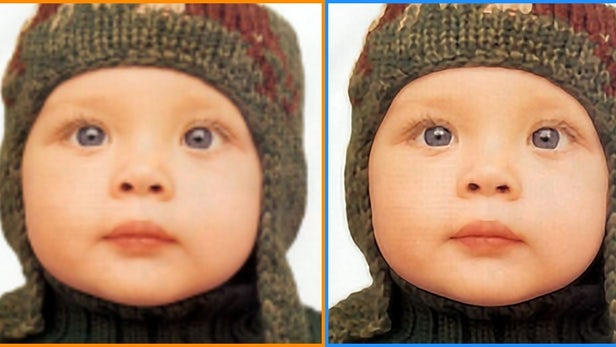
\includegraphics[width=\linewidth]{sr1.jpg}
    \caption{Blur correction}
    \label{fig:sr1} % insert suitable label, this is used to refer to a fig from within the text
\end{figure}

We also attempt to use capsule networks in place of convolutional neural networks to extract features. This should theoretically improve the feature extraction process since it has been shown that capsule networks are an improvement over conventional CNN networks.

\begin{figure}[htb]
    \centering
    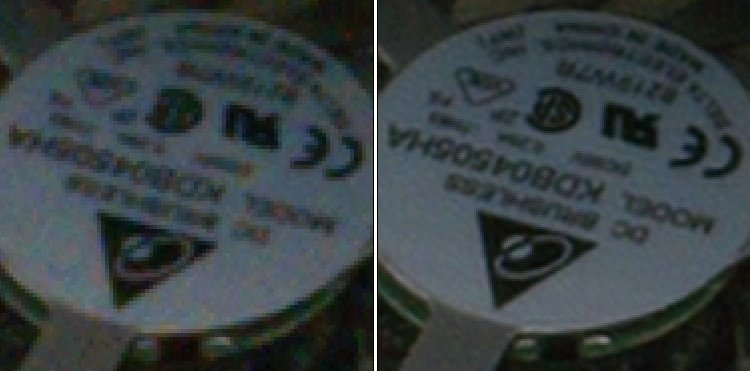
\includegraphics[width=\linewidth]{sr5.jpg}
    \caption{Better edge correction}
    \label{fig:sr5} % insert suitable label, this is used to refer to a fig from within the text
\end{figure}

Image Detail Reconstruction
In the case of data up - sampling, the transposed convolutional layer ( also known as a deconvolution layer ) proposed by Matthew D. Zeiler is typically used. T he t ransposed convolutional layer can learn up - sampling kernels, however, the process is similar to the usual convolutional layer and the reconstruction ability is limited. To obtain a better reconstruction performance, the transposed convolutional layers need to be stacked deeply , which means the process needs heavy computation. So we propose a parallelized CNN structure like the Network in Network, which usually consists of one (or more) 1x1 CNN(s). Remarkably, the 1x1 CNN layer 

\chapter{Module description}

The project can be essentially split into 3 main parts.

\begin{itemize}
\item Frontend module
\item Backend module
\item Image super resolution module
\end{itemize}

\section{Frontend module}

The frontend is the visual component of the system. It is the interface that the user will be interacting with. It will provide the user with a way to upload an image to the backend. It is also responsible for displaying the result of the image that has been worked on using the super resolution model once that is received back from the backend.
When a user uploads an image, the frontend encode it into base64 encoding and passes it over to the backend server. Once the image is received from the backend the frontend will parse it back from base64 to image and display in the UI.

\section{Backend module}

It is the API server. It serves as the glue code between the fronted and the Image super resolution model. It work be interacting with both of them. When a user uploads an image, it decodes the image from base64 and write it to an image file. This file is what the Image super resolution module reads. Not once the Image super resolution model is done with processing the image it then passes the image back to the backend. This image that is obtained from the Image super resolution model is then passed encoded into base64 encoding and sent back to the frotend.


\section{Image super resolution module}
It is the core of the system. This module does all the heavy lifting in this system. This is the part of the system that will do the actual transformation of the lower resolution image to the higher resolution image. It makes use of a \textbf{Deep Denoiseing Super Resolution (DDSRCNN)} model in order to do the same. It takes an image that has been written to disk by the backend, process it by initially cleaning it up then working on it using \textbf{Deep Denoiseing Super Resolution (DDSRCNN)} model. The processed image is then written back to the backend.

\chapter{Technology used}

\section{Image super resolution model}

\subsection{Tensorflow}
TensorFlow™ is an open source software library for high performance numerical computation. Its flexible architecture allows easy deployment of computation across a variety of platforms (CPUs, GPUs, TPUs), and from desktops to clusters of servers to mobile and edge devices. Originally developed by researchers and engineers from the Google Brain team within Google’s AI organization, it comes with strong support for machine learning and deep learning and the flexible numerical computation core is used across many other scientific domains

\subsection{Keras}
Keras is an open source neural network library written in Python. It is capable of running on top of TensorFlow, Microsoft Cognitive Toolkit, Theano, or MXNet. Designed to enable fast experimentation with deep neural networks, it focuses on being user-friendly, modular, and extensible. It was developed as part of the research effort of project ONEIROS (Open-ended Neuro-Electronic Intelligent Robot Operating System.

\section{Frontend}

\subsection{React}
React is a front-end library developed by Facebook. It is used for handling the view layer for web and mobile apps. ReactJS allows us to create reusable UI components. It is currently one of the most popular JavaScript libraries and has a strong foundation and large community behind it.

\section{Backend}

\subsection{Flask}
Flask is a microframework for Python based on Werkzeug and using Jinja2 for templating. It helps to easily prototype and iterate on various version of the backend api that is being provided.

\subsection{Gunicorn}
Gunicorn 'Green Unicorn' is a Python WSGI HTTP Server for UNIX. It's a pre-fork worker model. The Gunicorn server is broadly compatible with various web frameworks, simply implemented, light on server resources, and fairly speedy.

\chapter{Implementation}

\section{Flow chart}

\begin{figure}[htb]
    \centering
    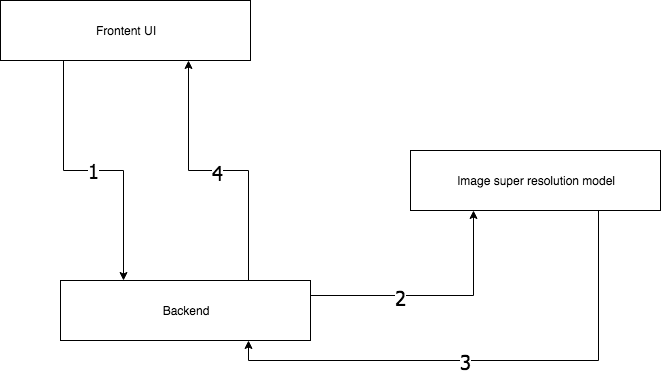
\includegraphics[width=\linewidth]{flow.png}
    \caption{Flow diagram}
    \label{fig:flow}
\end{figure}

\section {Overview of implementation}

The frontend is a React JavaScript app which provides a simple interface that allows user to upload any image in their computer or in their mobile device. The user uploaded image is then converted into a based64 encoded string and is passed on to the backend as a JSON through a POST request.

The backend is a Flask application that runs using Gunicorn. What we have in here is a simple web API that is expecting a POST request from the frontend with the content as the image that is to be converted and sent back. Flask provies us with a super simple and efficent API for creating web API's. Gunicorn lets up run Flask as a multithreaded web app handling all the multithreading heavylifing. When the backend recieves the image from the frontend as a API POST call from we convert that image from an bse64 encode string into a file.

This file is then fed into the Image super resolution model. The model is the core of the project and convets the image from a low resolution image into a high resolution image. This is done using a \textbf{Deep Denoiseing Super Resolution (DDSRCNN)} model. Once the model has done it's job of conveting the lower reolution image into a higher resolution image, it is sent back to the backend. The backend then encodes the new better image into a base64 encode string and sends it to the frontend.

The frontend service, once the result is received back from the bakend server will display that to the user and will have an option to download and store the image. The whole frontend is a completely static site which is hosted on a public static site hosting servie that is provide by surge.sh. The main advantage of hosting it on a public hosting service is that due to the availablility of CDN's (Content Delivery Network) arround the globe the page load speed will be very fast.

\section{Deep Denoiseing Super Resolution (DDSRCNN)}

The framework is fully convolutional (and deconvolutional. Deconvolution is essentially unsampling convolution). Rectification layers are added after each convolution and deconvolution. For low-level image restoration problems, we use neither pooling nor unpooling in the network as usually pooling discards useful image details that are essential for these tasks. It is worth mentioning that since the con- volutional and deconvolutional layers are symmetric, the network is essentially pixel-wise prediction, thus the size of input image can be arbitrary. The input and output of the network are images of the same size $w$ × $h$ × $c$, where $w$, $h$ and $c$ are width, height and number of channels.
Our main idea is that the convolutional layers act as a feature extractor, which preserve the primary components of objects in the image and meanwhile eliminating the corruptions. After forwarding through the convolutional layers, the corrupted input image is converted into a “clean” one. The subtle details of the image contents may be lost during this process. The deconvolutional layers are then combined to recover the details of image contents. The output of the deconvolutional layers is the recovered clean version of the input image. Moreover, we add skip connections from a convolutional layer to its corresponding mirrored deconvo- lutional layer. The passed convolutional feature maps are summed to the deconvolutional feature maps element-wise, and passed to the next layer after rectification. Deriving from the above architecture, we have used two networksvin our experiments, which are of 20 layers and 30 layers respectively, for image denoising, image super-resolution, JPEG deblocking and image inpainting.
\begin{figure}[htb]
    \centering
    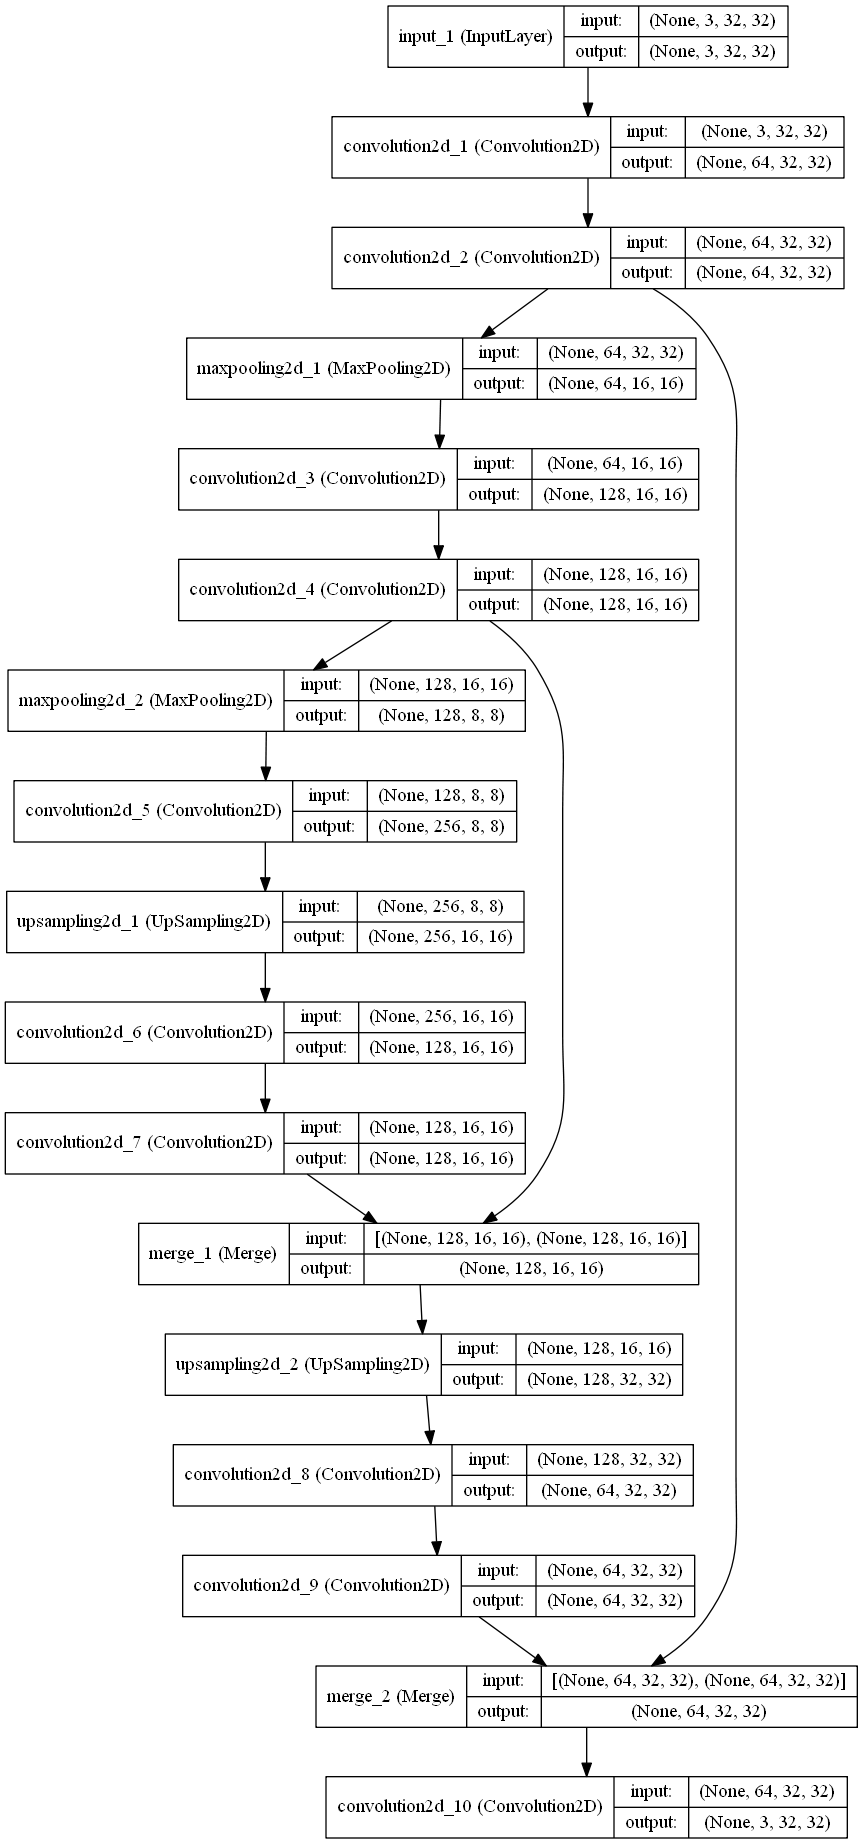
\includegraphics[width=\textwidth,height=15cm,keepaspectratio]{model.png}
    \caption{Deep Denoise model}
    \label{fig:modeldd}
\end{figure}

\chapter{System Requirements}

\section{Hardware requirements}

\begin{itemize}
    \item A UNIX based system
    \item 8 GB RAM
    \item NVDIA graphics card
\end{itemize}

\section{Software architecture}

\begin{itemize}
    \item Python
    \item Numpy
    \item Keras
    \item Tensorflow
\end{itemize}

% \chapter{Work progress}

\section{Phase 1: Literature Survey}

We have gone through the respective papers inorder to understand the working and implementaion of an Image Super Resolution system.

\bibitem{}Fast and Accurate Image Super Resolution by Deep CNN with Skip Connection and Network in Network,\ \url{https://arxiv.org/abs/1707.05425}

\bibitem{} Photo-Realistic Single Image Super-Resolution Using a Generative Adversarial Network\ \url{https://arxiv.org/abs/1609.04802}

\bibitem{}Image super-resolution: Historical overview
and future challenges\ \url{http://www.ifp.illinois.edu/~jyang29/papers/chap1.pdf}


\bibitem{}Image Super-Resolution Via Sparse Representation\ \url{http://ieeexplore.ieee.org/abstract/document/5466111}

\bibitem{}Image super-resolution as sparse representation of raw image patches\ \url{http://ieeexplore.ieee.org/abstract/document/4587647/}

\bibitem{}Image super-resolution using gradient profile prior\ \url{http://ieeexplore.ieee.org/abstract/document/4587659/}

\bibitem{}Single-Image Super-Resolution Using Sparse Regression and Natural Image Prior\ \url{http://ieeexplore.ieee.org/abstract/document/5396341/}

\bibitem{}Bayesian Image Super-Resolution \ \url{http://papers.nips.cc/paper/2315-bayesian-image-super-resolution.pdf}

\bibitem{}Learning a Deep Convolutional Network for Image Super-Resolution\ \url{https://link.springer.com/chapter/10.1007/978-3-319-10593-2_13}

\bibitem{}Super-resolution image reconstruction: a technical overview\ \url{http://ieeexplore.ieee.org/abstract/document/1203207/}

\section{Phase 2: Problem Statement}

We have anlysed the problem at hand inorder to improve how our system has to function in all the respects.

\section{Phase 3: System study}

We have been studying the existing system and finding out what we can adapt from them into our project inorder to improve how it works in both better resolution of images as well as faster way to generate images.

\section{Phase 4: Implementation}

We have been working on designing the final implementation of the research we have been on so far. We have been able to condense the research we have done so far into a simple and elegent solution that we can implement and has started with it.

\chapter{Future work}

The implemented system of image super resolution as of now is a good and stable platform for us to build future tools on top of this. We can have secific tools develeoped on top of this as well as make it a much more special purpose tool by adapting necessary changes such as selected dataset and image pre processing.

We do shoot a lot of blurry and generally bad images in our phone. We can use our system to provode a simple and intutivie process to change all those images into a better quality image. Another specific use case to which the project can be adapted to is the retrieval of more information from older and degraded photos. It will help us to better understand the historic photos.

We can also adapt the system to a specific use case, ie using it for images of text. This is a very important use of this project as it is hard to understand blurry text, but with this we can make use of image super resolution to make the text readable.
\chapter{Conclusion}

Image super-resolution is an important concept in image processing. The advent of deep learning his given the field a new method of attack for solving it. With it's application in forensic analysis to medical imaging, image super-resolution will continue to be an area of research in both image processing as well as deep learning.
\phantomsection
\addcontentsline{toc}{chapter}{References}
\begin{thebibliography}{99}

\bibitem{}Fast and Accurate Image Super Resolution by Deep CNN with Skip Connection and Network in Network,\ \url{https://arxiv.org/abs/1707.05425}

\bibitem{} Photo-Realistic Single Image Super-Resolution Using a Generative Adversarial Network\ \url{https://arxiv.org/abs/1609.04802}

\bibitem{}Image super-resolution: Historical overview
and future challenges\ \url{http://www.ifp.illinois.edu/~jyang29/papers/chap1.pdf}


\bibitem{}Image Super-Resolution Via Sparse Representation\ \url{http://ieeexplore.ieee.org/abstract/document/5466111}

\bibitem{}Image super-resolution as sparse representation of raw image patches\ \url{http://ieeexplore.ieee.org/abstract/document/4587647/}

\bibitem{}Image super-resolution using gradient profile prior\ \url{http://ieeexplore.ieee.org/abstract/document/4587659/}

\bibitem{}Single-Image Super-Resolution Using Sparse Regression and Natural Image Prior\ \url{http://ieeexplore.ieee.org/abstract/document/5396341/}

\bibitem{}Bayesian Image Super-Resolution \ \url{http://papers.nips.cc/paper/2315-bayesian-image-super-resolution.pdf}

\bibitem{}Learning a Deep Convolutional Network for Image Super-Resolution\ \url{https://link.springer.com/chapter/10.1007/978-3-319-10593-2_13}

\bibitem{}Super-resolution image reconstruction: a technical overview\ \url{http://ieeexplore.ieee.org/abstract/document/1203207/}

\end{thebibliography}

\phantomsection
\addcontentsline{toc}{chapter}{Appendices}

\section{Appendices A ( Screenshots )}

\begin{figure}[htb]
    \centering
    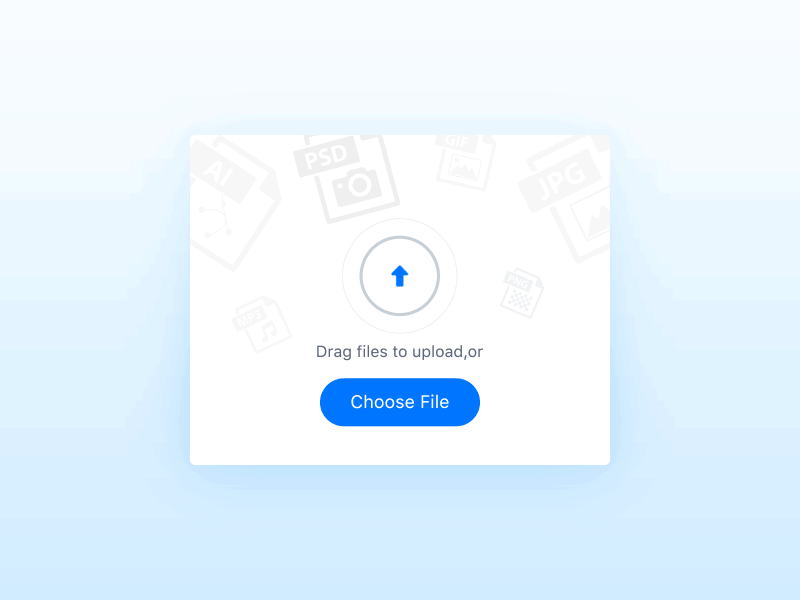
\includegraphics[width=\textwidth]{up.png}
    \caption{Upload screen}
    \label{fig:modeldd}
\end{figure}

\begin{figure}[htb]
    \centering
    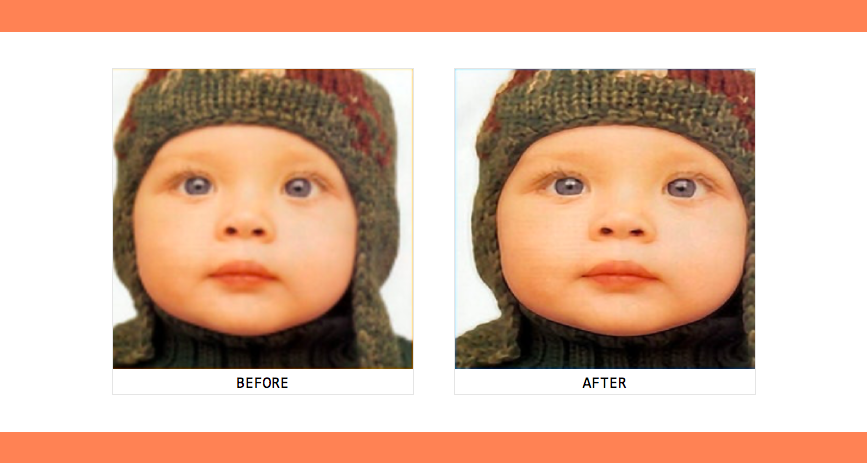
\includegraphics[width=\textwidth]{shot.png}
    \caption{Image result screen}
    \label{fig:modeldd}
\end{figure}

\section{Appendices B ( Source Code )}

\subsection{Python Flask POST}

\lstinputlisting[language=python]{code/flask.py}

\subsection{React component}

\lstinputlisting[language=javascript]{code/react.js}

\subsection{Keras model}

\lstinputlisting[language=python]{code/model.py}

\end{document}
